\documentclass{standalone}

\usepackage{tikz}
\usetikzlibrary{decorations.markings}
\begin{document}



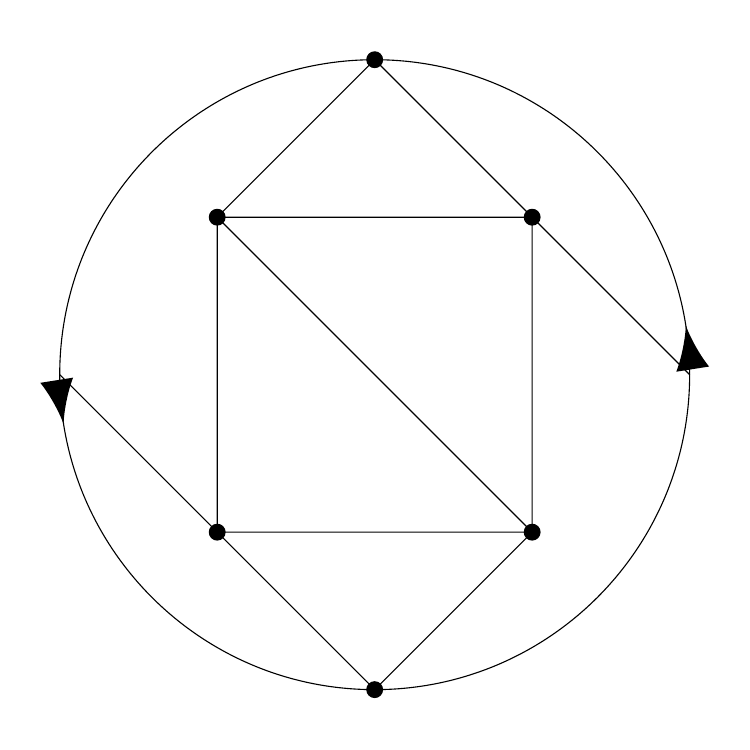
\begin{tikzpicture}[scale=2]

\draw[white] (-2.2,-.2)--(-2.2,-.2);
\draw[white] (2.2,4.2)--(2.2,4.2);

\draw[ 
        decoration={markings, mark=at position 0.55 with {\arrow[scale=4]{latex}}},     postaction={decorate}
        ] (0,0) arc (-90:90:2);
\draw[        decoration={markings, mark=at position 0.55 with {\arrow[scale=4]{latex}}},     postaction={decorate}] (0,4) arc (90:270:2);
\filldraw (0,0) circle (.05cm);
\filldraw (0,4) circle (.05cm);

\filldraw (-1,1) circle (.05cm);
\filldraw (-1,3) circle (.05cm);
\filldraw (1,1) circle (.05cm);
\filldraw (1,3) circle (.05cm);

\draw (0,4)--(1,3)--(1,1)--(0,0)--(-1,1)--(-1,3)--(0,4);
\draw (-2,2)--(-1,1)--(1,1)--(-1,3)--(1,3)--(2,2);


\end{tikzpicture} 


\end{document}
